\documentclass[../ProgettoTecWeb2.tex]{subfiles}

\begin{document}
\section{L'homepage}
	\begin{figure} [h]
			\centering
			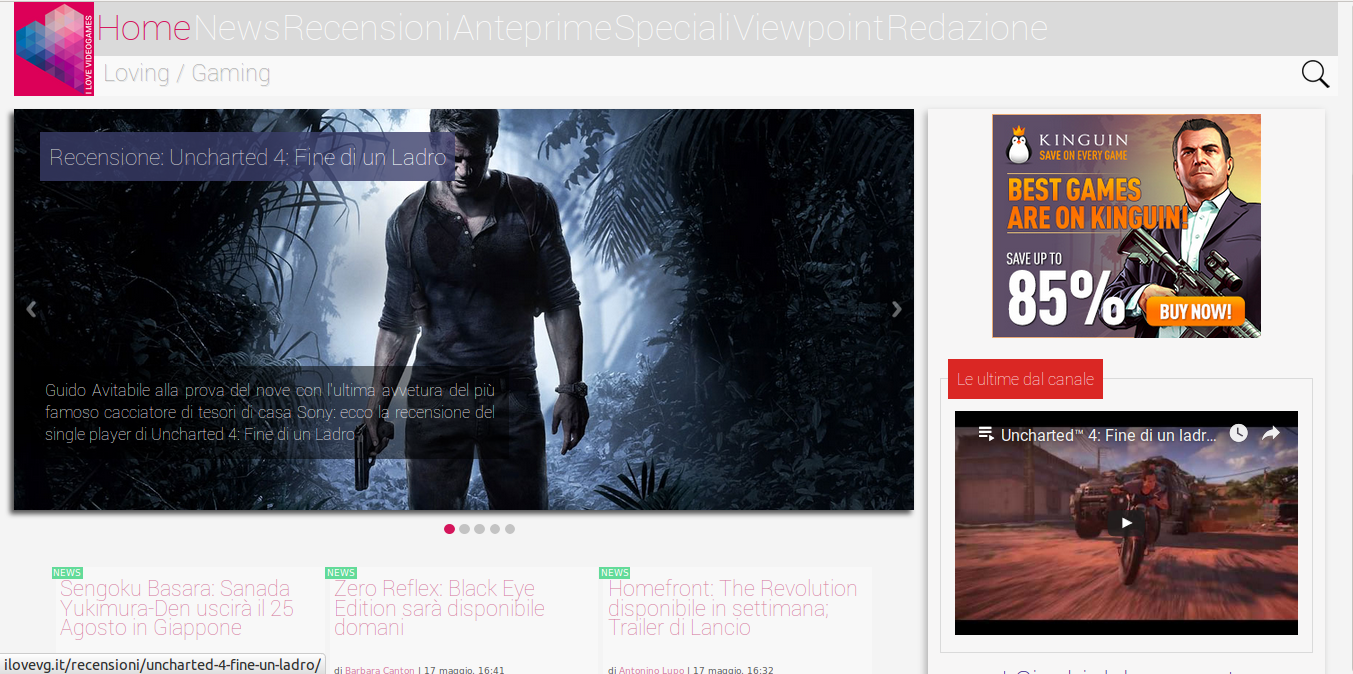
\includegraphics[scale=0.3]{img/ScreenHomePage}
			\caption{Homepage del sito}
			\label{fig:AprireProgetto}
		\end{figure}
	\subsection{Le 6 w}
		L'homepage di un sito web dovrebbe sempre rispondere alle 6 w giornalistiche, un po' riadattate al contesto del web.
		\subsubsection{Where}
			L'asse \textit{where} indica in che tipo di sito sono arrivato. Il primo impatto già ci fornisce indicazione sul contenuto del sito web difatti troviamo la prima pagina disseminata di immagini di videogiochi. Sotto il menù troviamo una grande scritte che recita \textit{Loving / Gaming} ed inoltre nella colonna a sinistra troviam il link al canale youtube associato al sito web, che presenta video di gameplay, ed una lista dei giochi del momento. Anche la pubblicità in alto nella colonna di destra aiuta a capire il contesto poichè rimanda ad un altro sito web per la vendita di videogiochi.
		\subsubsection{Who}
			L'asse \textit{who} indica chi rappresenta il sito web. In alto a sinistra è possibile vedere il logo del sito web con vicino il nome. Tale logo segue il menu nel caso di scroll nella pagina e quindi è sempre visibile. Il nome forse è un po' troppo piccolo. Nel menù inoltre è presente il link per arrivare alla sezione \href{http://ilovevg.it/redazione/}{Redazione}. Tale sezione presenta in modo ironico le persone che collaborano al sito web e quindi a chi rappresenta realmente il sito.
		\subsubsection{Why}
			L'asse \textit{why} deve esporre i benefici del sito web. Come sopra citato il sito si occupa di recensioni e notizie riguardanti il mondo dei videogiochi. Tale asse è soddisfatto dalle scritte sopra le immagini che recitano ``Recesione:'' seguito dal nome del gioco e dai riquadri delle notizie che in alto a sinistra hanno un riquadro che comprende la scritta \textit{news}. L'asse è poi soddisfatto anche dal menu che comprende le voci:
			\begin{itemize}
				\item News;
				\item Recensioni;
				\item Anteprime;
				\item Speciali;
				\item Redazione.
			\end{itemize}
		\subsubsection{What}
			L'asse \textit{what} indica cosa il sito offre. Le offerte del sito web sono abbastanza evidenti: infatti subito si vedono le immagini relative alle notizie e recensioni principali. Scendendo nella pagina poi si possono vedere altre notizie e recensioni. Inoltre l'identificazione di tale asse è semplificata dal menù.
		\subsubsection{When}
			L'asse \textit{when} indica le novità temporali relative al sito. 
		\subsubsection{How}
\end{document}
